In this section, we first introduce the design principles of \xxx (Section \cref{principles}). Then we present the topology of the network (Section \cref{topo}), how the structure is formed (Section \cref{formation}) and maintained (Section \cref{maintain}), and the broadcast algorithm (Section \cref{broadcast}). Security issues are also addressed in the design of \xxx (Section \cref{security}).

\subsection{Design Principles} \label{principles}

The design of \xxx as a Peer-to-Peer network layer under a blockchain system follows four principles:
\noindent
\begin{itemize}[noitemsep, topsep=0pt]
	\item Fair: An unfair P2P network may ascend free-riders, frustrate majority of users and consequently lead to instability of the network \cite{naghizadeh2016improving}.
	\item Self-organizing: No central server should be responsible for organizing the structure of the network. In other words, the decentralization nature of the P2P network should not be affected.
	\item Anonymous: Each node in the network and the network topology should be hidden from the outsider so that target attack can be avoided to some extent.
	\item Robust in the dynamic environment: The network is unstable due to the frequent disconnection or node-join. The structure of the network should be easy to maintain in a distributed manner.
\end{itemize}

%\item Efficient on broadcast: The converge time of each message to broadcast should be as small as possible. Therefore, the number of concurrent messages on flight will be reduced.
%\item Scalable to large number of nodes: The P2P network should be able to scale up to tremendous number of nodes as a public block chain may grow up to millions of nodes.

\subsection{Topology} \label{topo}

Before presenting the protocol, several key concepts should be defined clearly:
\begin{itemize}[noitemsep, topsep=0pt]
	\item Node: One instance of a server/virtual machine in the network;
	\item Ring: A group of nodes connected in a ring-like structure.
	\item Contact Node: the node on the ring who is in charge of adding new nodes, contacting the nodes in the upper level of the network, and broadcasting the message.\\
\end{itemize}

\begin{figure}[t]
	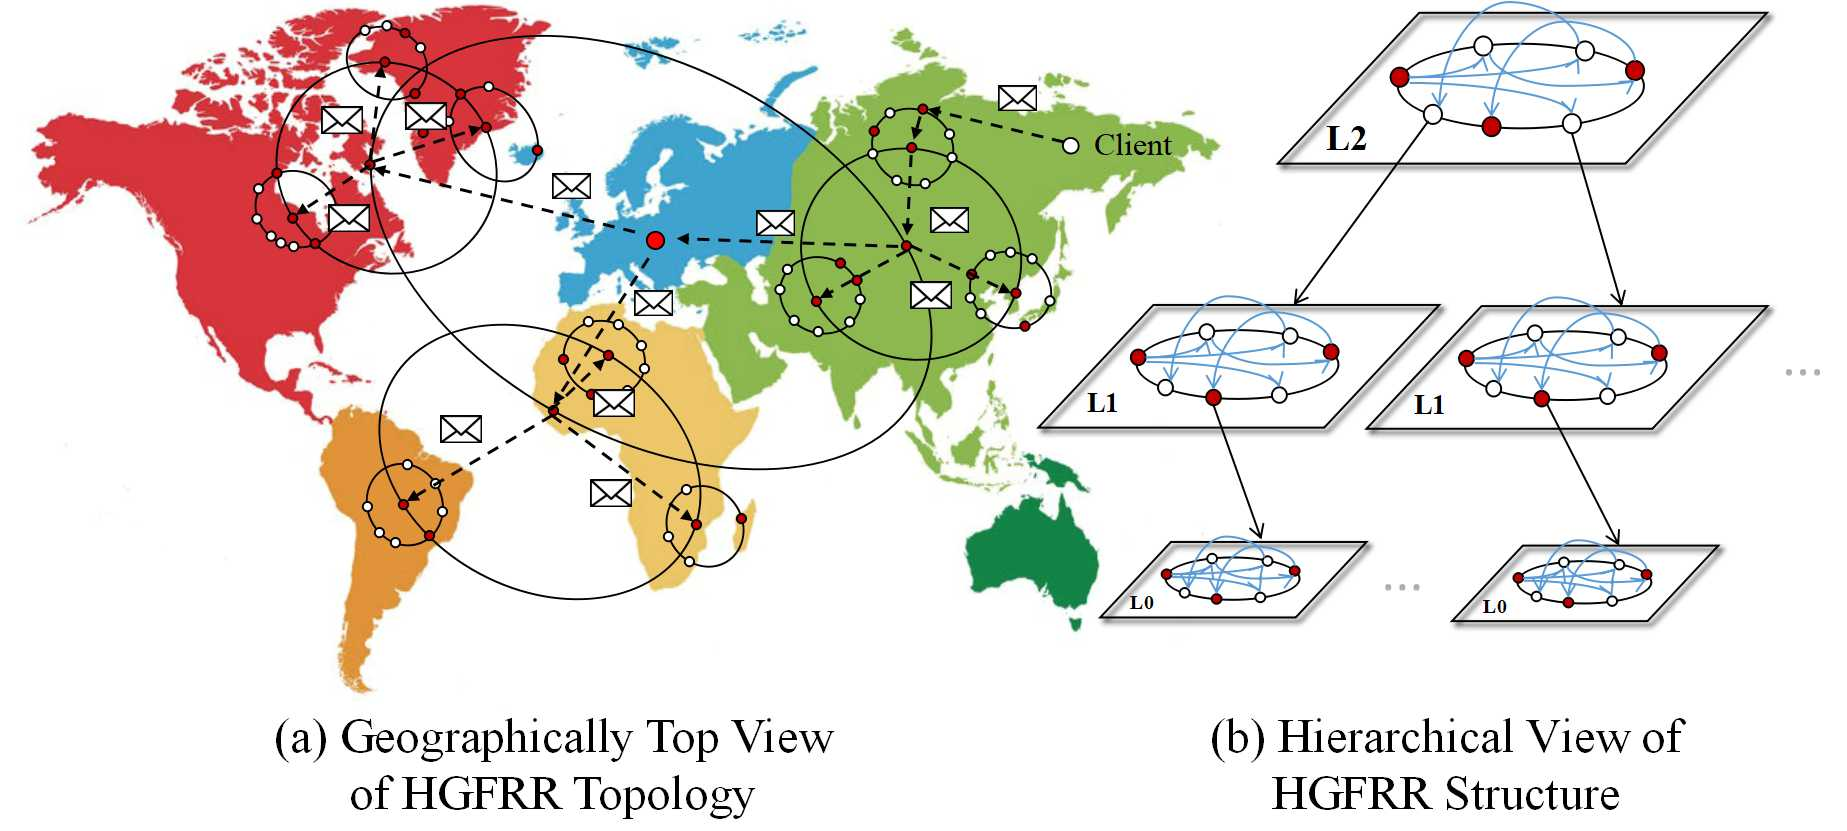
\includegraphics[width=0.47\textwidth]{figures/topo.jpg}
	\caption{Topology Illustration of a 3-level \xxx Network}
	\label{fig:topo}
\end{figure}

The network topology of \xxx is basically a fractal-ring structure, where lower level rings reside on higher level rings (See Figure \ref{fig:topo}) in a recursive way. At the top level resides the largest ring where several sub-ring resides on while at the bottom level resides the smallest rings. The figure shows a network of 3 levels. Level 2 contains the largest ring. On the largest ring, there are three sub-rings of 2 levels. Level 1 contains the second largest rings and level 0 contains the smallest rings. The nodes in red are contact nodes of each ring. They are elected to be normal nodes of the upper level ring.

\subsubsection{Structure Formation} \label{formation}

When a new node wants to join the network, it will first send ping-messages to each of the contact nodes of the largest ring (at the top level). The new node will pick the contact node with the shorted response time to send a join-message. The contact node will then decide which sub-ring it should add this new node to, by sending the node information of contact nodes of each sub-ring back to the new node. Recursively, the new node will then choose the sub-ring which is optimal in terms of response time. And the contact node of the sub-ring will then introduce the new node to the sub-sub-ring. In the end, the contact node of a ring at the bottom level will then add the new node to the ring. If the number of node on the ring that the new node join to exceeds the threshold, then this ring will transform to a two-level ring (See Figure TODO), i.e. several groups of nodes on the large ring will form several rings. The transformation will be further elaborated in Section \cref{maintain}. After a new node joins the network, the contact node of this ring will broadcast within ring this node's information. The member nodes of this ring will then tell their information by sending welcome-messages to the new node.

The upper level rings are formed by contact node election. When a ring is first formed, the first member node of the ring will be the contact node of this ring. Each generation of contact nodes have their term of service. At the end of the term, one of the contact nodes will generate random IDs from all member node IDs. This election result will be dispersed within ring, and multi-casted to the contact nodes of the upper level ring and the lower level rings.

\begin{figure}[t]
	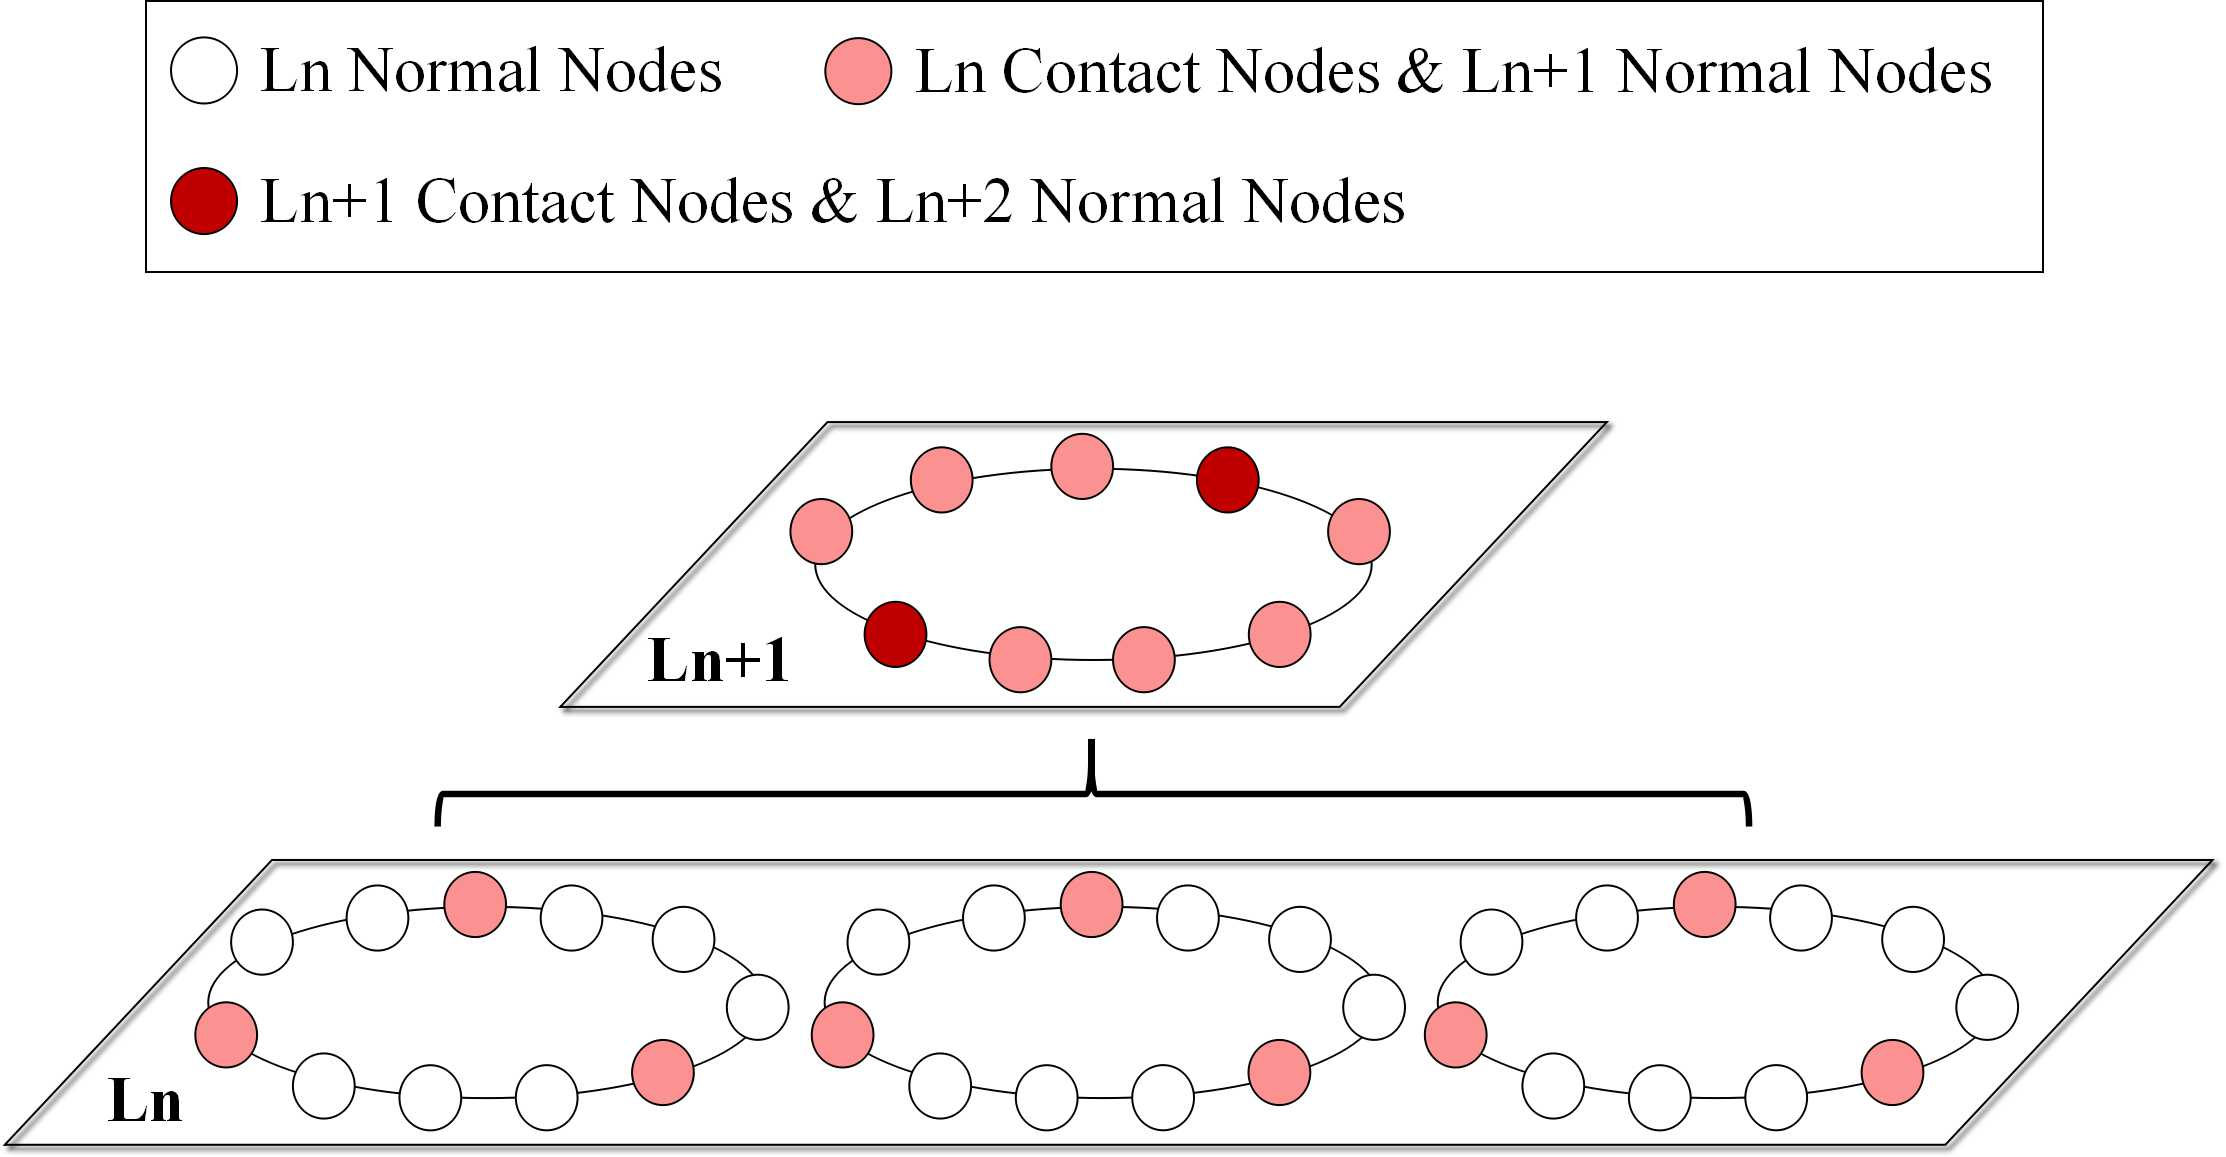
\includegraphics[width=0.47\textwidth]{figures/topo-vertical.jpg}
	\caption{Vertical Illustration of \xxx Network Structure. The figure illustrated the relationship between two levels next to each other.}
	\label{fig:topo}
\end{figure}

\begin{algorithm}
	\caption{Bootstrap}\label{euclid}
	\begin{algorithmic}[1]
		\Procedure{Node Join}{}
		\State $\var{response} \gets \var{queryDNSSeeds}()$
		\State $\var{contactNodeList} \gets \var{response.nodes}$
		\State $\var{level} \gets \var{response.topLevel}$
		\BState \emph{loop}:
		\If {$\var{level} = \var{0}$}
		\State $\textbf{break}$
		\Else
		\State $\var{optimalMetric} \gets \var{0}$
		\For {$\var{contactNode} : \var{contactNodeList}$}
		\State $\var{metric} \gets \var{testProximity}(\var{contactNode})$
		\If {$\var{metric} > \var{optimalMetric}$}
		\State $\var{optimalMetric} \gets \var{metric}$
		\State $\var{targetNode} \gets \var{contactNode}$
		\EndIf
		\EndFor
		\State $\var{response} \gets \var{queryNode}(\var{contactNode}, \var{level})$
		\State $\var{contactNodeList} \gets \var{response.nodes}$
		\State $\var{level} \gets \var{level}\var{-1}$
		\State \textbf{goto} \emph{loop}.
		\EndIf
		\State $/* \text{contact node of level 0 ring broadcast node-join}$
		\State $\text{\; * message withing the ring */}$
		\State $\var{this.}\var{nodeTable.insert}(\var{recvMsg.node})$
		\If {$\var{recvMsg.node.contactNode} = \var{true}$}
		\State $\var{contactNode} \gets \var{recvMsg.node}$
		\State $\var{contactNodeList.insert}(\var{contactNode})$
		\EndIf
		\EndProcedure
	\end{algorithmic}
\end{algorithm}

\subsubsection{Structure Maintenance} \label{maintain}

Each node on the bottom ring will send heart-beat messages to its successor and predecessor to check the aliveness of them. Once a node are not responding to the heart-beat message after the timeout value, the node will double check the liveness of this node with its, e.g. if A's predecessor B does not respond, A will check with the predecessor of B. If they agree that this node left the network (intentionally or accidentally), the information will be disseminated to the ring and this node will be officially removed from the network. If the missing node is the contact node, then the next generation of contact nodes will be elected. If the number of nodes on the ring is smaller than the lower limit, a transformation from right to left in Figure [TODO] will be performed.

\iffalse
\begin{algorithm}
	\caption{Maintenance}\label{euclid}
	\begin{algorithmic}[1]
		\State {\text{// This function will be called every \var{TIME\_INTERVAL}}}
		\Function{detect\_node\_left}{}
		\If{$\var{liveness\_check\_predecessor}() = \var{false}$}
		\State $\var{msg} \gets \var{constructNodeLeaveMSG}()$
		\State $\var{this.inRingBroadcast(msg)}$
		\EndIf
		\If{$\var{liveness\_check\_successor}() = \var{false}$}
		\State $\var{msg} \gets \var{constructNodeLeaveMSG}()$
		\State $\var{this.inRingBroadcast(msg)}$
		\EndIf
		\EndFunction
		\\
		\Function{liveness\_check\_predecessor}{}
		\State $\var{ret} = \var{sendHeartBeatMSG(this.predecessor)}$
		\If{$\var{ret.type} = \var{TIMEOUT}$}
		\State $\var{status} \gets \var{confirmWithPrePredecessor}()$
		\State \Return $\var{status}$
		\EndIf
		\EndFunction
		\\
		\Function{liveness\_check\_successor}{}
		\State $\var{ret} = \var{sendHeartBeatMSG(this.successor)}$
		\If{$\var{ret.type} = \var{TIMEOUT}$}
		\State $\var{status} \gets \var{confirmWithSucSuccessor}()$
		\State \Return $\var{status}$
		\EndIf
		\EndFunction
	\end{algorithmic}
\end{algorithm}
\fi

\subsection{Broadcast} \label{broadcast}

\textbf{Broadcast} is the process of disseminating a message from any node to the whole network. When a node wants to send a message to the whole network, it will first send broadcast-message to one of the contact nodes of the ring it resides on. Then the message will be routed to two directions: one direction is downwards, i.e. the contact node will broadcast the message in the ring and recursively in the sub-rings; the other direction is upwards, i.e. the contact node will send broadcast-message to one of the contact nodes of the upper level ring. Recursively, the broadcast-message will be received by one of the contact nodes of the largest ring. Then the contact node will broadcast recursively in the sub-rings. Till the bottom level, each node in the fractal ring will receive this message.

The k-ary distributed spanning tree method \cite{el2003efficient} is used to broadcast message in a ring. Details will be presented in the subsection. Based on this method, the time complexity of a broadcast operation will be $O(logN)$ and message complexity will be $(O(N))$, which are currently the best among related works.

\subsubsection{Broadcast Within-Ring Mechanism}

In-ring broadcast is based on the k-ary distributed spanning tree method. The basic idea is that the broadcast starter will first generate a random number $k$, and then a k-ary spanning tree can be formed in a distributed manner. Broadcast will then be triggered from the root to every node in the tree. The reason we choose to randomize the parameter k is that the network should be hidden from the attacker. If it keeps using the same parameter k, the routing pattern will be known easily by watching the network activities for a long time. The spanning tree are formed by using the broadcaster (which is numbered 0) as the root. Node 0 will connect to node $0+k^0$, $0+k^1$, $0+k^2$, and so on. Similarly, node 1 will connect to $1+k^0$, $1+k^1$, $1+k^2$, and so on. The pattern is: node $i$ will connect to $i+k^0$, $i+k^1$, $i+k^2$, and so on. The overall time complexity of this method will be $O(logN)$, where $N$ is the number of nodes in the ring.

\begin{lstlisting}
// broadcast data from any node in the network
void broadcast(data) {
  level = 0;
  contactNode = selectFromContactNodes(level);
  msg = wrapMsg(data);
  sendTo(contactNode, msg);
  return;
}

// broadcast upwards
void broadcast_up(currLvl, data) {
  level = currLvl + 1;
  contactNode = selectFromContactNodes(level);
  msg = wrapMsg(data);
  sendTo(contactNode, msg);
  return;
}

// broadcast within ring
void broadcast_down(currLvl, msg) {
  endID = this.getNodeTableSize(currLvl);
  i = 0;
  nodeOrder = msg.nodeOrder;
  k = msg.k;
  while (nodeOrder + pow(k, i) < endID) {
    i++;
    if (pow(k, i) <= nodeOrder) {
      continue;
    } else {
      targetID = nodeOrder + pow(k, i);
      if (targetID > endID)
        targetID -= endID + 1;
      receiver = this.getPeer(targetID, currLvl);
      msg = wrapMsg(msg);
      sendTo(receiver, msg);
    }
  }	
  return;
}
\end{lstlisting}

\iffalse
\begin{algorithm}[t]
	\caption{Broadcast}\label{broadcast}
	\begin{algorithmic}[1]
		\Function{broadcast}{\var{data}}
		\State $\var{level} \gets \var{0}$
		\State $\var{contactNode} \gets \var{selectFromContactNodes(level)}$
		\State $\var{message} \gets \var{wrapMessage(data)}$
		\State $\var{sendTo(contactNode, message)}$
		\EndFunction
		\\
		\Function{broadcast\_up}{\var{currentLevel, data}}
		\State $\var{level} \gets \var{currentLevel+1}$
		\State $\var{contactNode} \gets \var{selectFromContactNodes(level)}$
		\State $\var{message} \gets \var{wrapMessage(data)}$
		\State $\var{sendTo(contactNode, message)}$
		\EndFunction
		\\
		\Function{broadcast\_within\_ring}{\var{currentLevel, message, sentIDs, k}}
		\State $\var{endID} \gets \var{this.getNodeTableSize(currentLevel)}$
		\State $\var{i} \gets \var{0}$
		\State $\var{nodeOrder} \gets \var{message.nodeOrder}$
		\While {$\var{nodeOrder + pow(k, i)} < \var{endID}$}
		\State $\var{currentID = nodeOrder + pow(k, i)}$
			\If{$\var{pow(k, i) <= nodeOrder}$}
			\State $\var{i++}$
			\State $\textbf{continue}$
			\Else
			\State $\var{targetNodeID = NodeID + pow(k, i)}$
			\If{$\var{targetNodeID > endID}$}
			\State $\var{targetNodeID -= endID + 1}$
			\EndIf
			\State $\var{args=(targetNodeID, currentLevel)}$
			\State $\var{receiver} \gets (\var{this.getPeer(args)})$
			\State $\var{i++}$
			\State $\var{sendTo(receiver, message)}$
			\EndIf
		\EndWhile
		\EndFunction
	\end{algorithmic}
\end{algorithm}
\fi

\subsection{Security Consideration} \label{security}

\xxx uses Intel SGX attestations to build trust base among blockchain nodes. The routing information are well saved by Intel SGX enclaves. The behavior of each node after receiving a message or when sending a message are protected by the enclaves. In addition, the parameter k used in within-ring broadcast and the IDs of the contact nodes are randomly generated by using Intel SGX \texttt{sgx\_read\_rand} API.

To hide the existence of \xxx contact nodes from outsiders, there are two mechanisms. First, fake messages are used to make the behavior of a contact node the same with that of a normal node. For a contact node, it will send messages of the same size to both one of the contact nodes and some of the past contact nodes in the upper level ring. For a normal node, it will send messages of the same size to both one of the contact nodes and some of its peers in the same level ring. When broadcasting messages withing the ring, the random parameter k will hide the relative orders of each node. Apart from broadcasting to its children in the constructed k-ary distributed spanning tree, each node will randomly choose a node to send fake message. All fake messages are of the same size of the real messages. Hackers may watch the packets sending out from a node and sending to the node for a long time. However, during one contact node service term, no difference can be discovered from the data collected. Second, contact nodes of a ring will be elected for every service term. One contact node of the last service term will generate random IDs by using Intel SGX's \texttt{sgx\_read\_rand ()} function \cite{costan2016intel}, and then broadcast the nomination result withing the ring. Due to both limited contact node service term period and the same behavior during one service term, outsider cannot differentiate contact nodes from normal nodes. \xxx's network topology and structure are well hidden from the outsiders. Packet analysis is done by using WireShark and the evaluation result is discussed in Section [TODO].